\documentclass{amia}
\usepackage{graphicx}
\usepackage[labelfont=bf]{caption}
\usepackage[superscript,nomove]{cite}
\usepackage{color}
\usepackage{amssymb}
\usepackage{hyperref}
\usepackage{multirow}
\usepackage{subfigure}
\usepackage{amsmath}
\geometry{left=1.5cm, top=0.8cm, right=1.5cm, bottom=1.0cm, footskip=1.5cm} % Configure page margins with geometry

\hypersetup{
    colorlinks=true,
    linkcolor=blue,
    filecolor=magenta,      
    urlcolor=cyan,
    citecolor = black
}
\begin{document}

\title{Trading Strategy Project}

\author{Yan Jiang}

%\author{Yan Jiang, Degrees$^{1}$}
\institutes{
%    $^1$Institution, City, State, Country (if applicable); $^2$Institution, City, State, Country (if applicable)\\
}

\maketitle

\textit{This is code part: \href{https://github.gatech.edu/yxie351/CSE6250-Healthcare-SleepData}{Git Repo Link (https://github.gatech.edu/yxie351/CSE6250-Healthcare-SleepData)}}

\section*{Goal}
This project focuses on building trading strategies for JPM to maximize our portfolio value. 

\section*{Introduction}
The project contains two parts: (1) trained JPM data starting with \$100,000 cash using manual strategy (MS) and strategy learner (Q-Learning) (SL) to generate best tradings strategy in in-sample (2008/1/1 - 2009/12/31) and tested it in out-of-sample (2010/1/1 - 2011/12/31). There only were three allowable positions: 1000 shares long, 1000 shares short and 0 shares; (2) evaluated those two strategies by calculating daily portfolio value based on strategy-generated tradings and then computing cumulative return, mean of daily return and standard deviation of daily return for them. Benchmark was also created to compare with our strategies. Benchmark also started with \$100,000, investigated 1000 shares on the first trading day and held that position. This report will interpret strategy building processes and display a chart to evaluate those two strategies. The code and related files can be found through this link: \textit{\href{https://github.gatech.edu/yxie351/CSE6250-Healthcare-SleepData}{Git Repo Link (https://github.gatech.edu/yxie351/CSE6250-Healthcare-SleepData)}}


\subsection*{Strategy Building}
In this project, Strength Index (RSI), Bollinger Bands B\% (BBP) and Commodity Channel Index (CCI) were selected to build manual strategy (MS) and strategy learner (Q-Learning) (SL). 
In manual strategy, BBP, RSI, and CCI were calculated and different values were assigned to each of them at their different conditions as below:
\vspace{-3mm}
\begin{figure}[H]
	\centering
	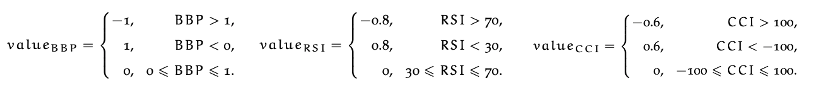
\includegraphics[height=1.5cm]{pics/ms_val.png}
	%\captionsetup{justification = centering}
	%\caption{Benchmark vs. Manual Strategy vs. Strategy Learner in Portfolio Values (In-sample period)}
	%\label{fig:figure4}
\end{figure}
\vspace{-5mm}
Those criterions I selected in this study are usually applied in stocking analytics as described in section. Those values were summed up as each day indication and made long/short/hold decision based on this indication value:
\vspace{-3mm}
\begin{figure}[H]
	\centering
	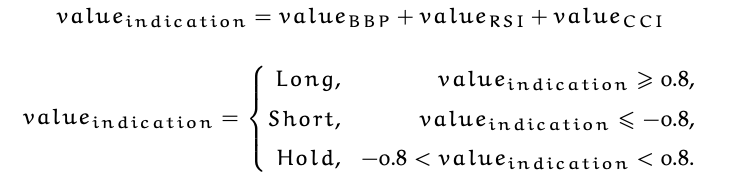
\includegraphics[height=1.8cm]{pics/ms_formula.png}
	%\captionsetup{justification = centering}
	%\caption{Benchmark vs. Manual Strategy vs. Strategy Learner in Portfolio Values (In-sample period)}
	%\label{fig:figure4}
\end{figure}
\vspace{-5mm}
In strategy learner, Q-learning was used to frame this trading strategy. Combined stock trading processes and project requirements, three factors were defined: (1) actions: 1) long 1000 shares, 2) short 1000 shares, 3) holding; (2) states: discretized RSI in to 8 intervals, BBP into 10 intervals, CCI into 8 intervals, and permutated all intervals. Therefore, there are 8*8*10=640 states. Those states were assigned to each day according to daily RSI, BBP, and CCI intervals combination; (3) rewards: daily return. In the Q-learning, for each day (day loop): (1) calculates indicators and then get a state; (2) request action based on this state by querying current Q table (find a action with maximum rewards) (3) calculate reward based requested action at this state and update reward based on step (3) reward and step (2) state in Q table; repeat above day loop multiple times until cumulative return stops improving. 

\subsection*{Strategy Evaluation}
In order to evaluate manual strategy and strategy learner, impact of 0.005, commission of \$9.95, and start value of \$100,000 were used, and the daily portfolio values were normalized for benchmark, manual strategy and strategy learner.The Figure 1 presents normalized portfolio values for benchmark, manual strategy and strategy learner. 
\vspace{-1mm}
\begin{figure}[H]
	\centering
	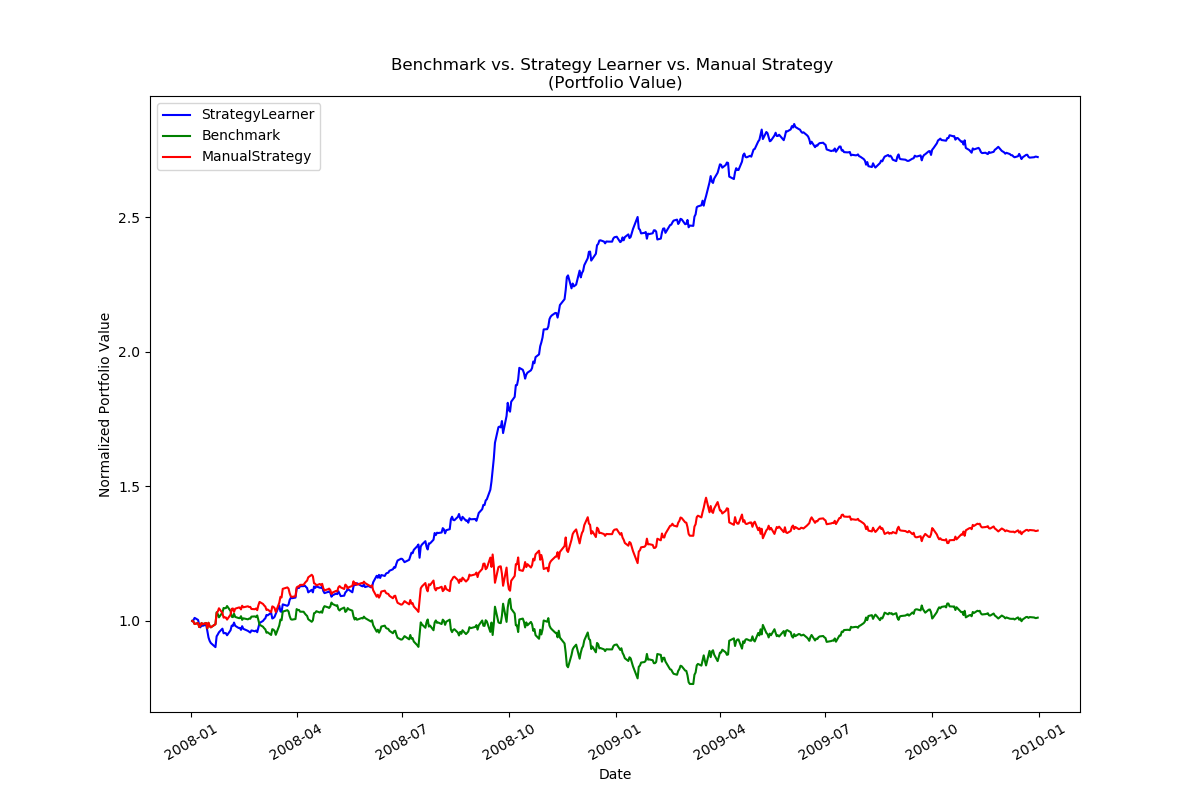
\includegraphics[height=4cm]{pics/exp1.png}
	%\captionsetup{justification = centering}
	\caption{Benchmark vs. Manual Strategy vs. Strategy Learner in Portfolio Values}
\end{figure}

\end{document}

